\begin{figure}[b]
	\begin{minipage}{\linewidth}
		\centering
		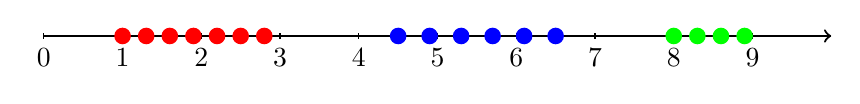
\begin{tikzpicture}
		\draw[thick,->] (0,0) -- (10,0);
		\foreach \x in {0,...,9} \draw (\x cm,1pt) -- (\x cm,-1pt) node[anchor=north] {$\x$};
		
		\foreach \x in {0,0.3,...,2} \fill[red](\x+1,0) circle (3pt);
		\foreach \x in {0,0.4,...,2} \fill[blue](\x+4.5,0) circle (3pt);
		\foreach \x in {0,0.3,...,1} \fill[green](\x+8,0) circle (3pt);
		
		\end{tikzpicture}
		\subcaption{Grupy}\label{odc:dbscan:groups}
	\end{minipage}
	\linebreak
	\linebreak
	\linebreak
	\begin{minipage}{\linewidth}
		\centering
		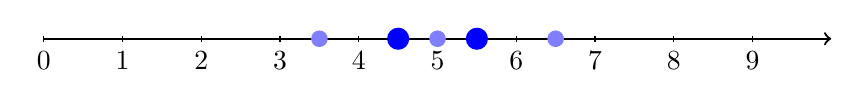
\begin{tikzpicture}
		\draw[thick,->] (0,0) -- (10,0);
		\foreach \x in {0,...,9} \draw (\x cm,1pt) -- (\x cm,-1pt) node[anchor=north] {$\x$};

		\fill[blue!50](3.5,0) circle (3pt);
		\fill[blue](4.5,0) circle (4pt);
		\fill[blue!50](5,0) circle (3pt);
		\fill[blue](5.5,0) circle (4pt);
		\fill[blue!50](6.5,0) circle (3pt);
		 
		\end{tikzpicture}
		\subcaption{Punkty brzegowe(mniejsze) i rdzeniowe, $ \varepsilon=1 $, $ \mu=4 $}\label{odc:dbscan:edge-points}
	\end{minipage}
	\caption{DBSCAN w jedno-wymiarowej przestrzeni.}
\end{figure}
